% SOURCE: Zarko @ Stackoverflow - https://tex.stackexchange.com/questions/250882/tikz-to-draw-timeline-for-infectious
\documentclass{article}
\usepackage{tikz}
\usetikzlibrary{arrows,positioning,decorations.pathreplacing}

\begin{document}
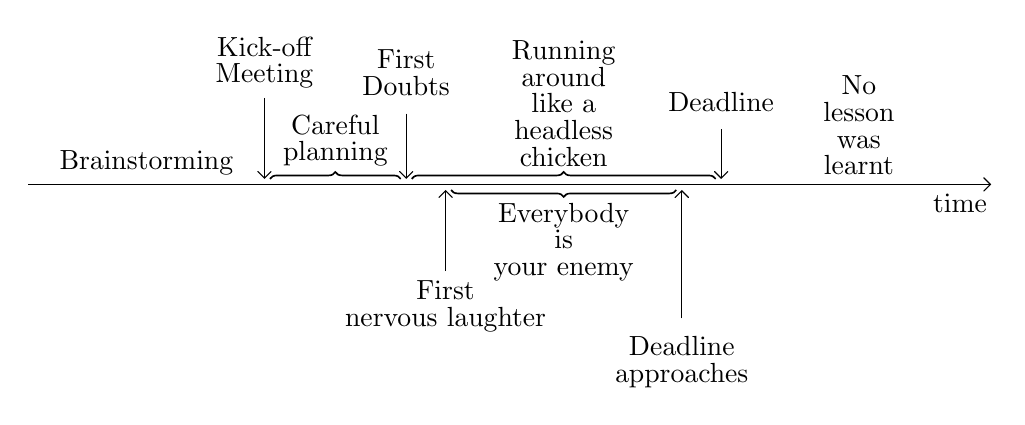
\begin{tikzpicture}[
	every node/.style = {align=center},
	Line/.style = {-angle 90, shorten >=2pt},
	Brace/.style args = {#1}{semithick, decorate, decoration={brace,#1,raise=2pt,
		pre=moveto,pre length=2pt,post=moveto,post length=2pt,}},
		ys/.style = {yshift=#1}
]
\linespread{0.8}
\coordinate (a) at (0,0);
\coordinate[right=30mm of a]    (b);
\coordinate[right=18mm of b]    (c);
\coordinate[right= 5mm of c]    (d);
\coordinate[right=30mm of d]    (e);
\coordinate[right= 5mm of e]    (f);
\coordinate[right=35mm of f]    (g);

\draw[Line] (a) -- node[above] {Brainstorming}    (b) -- (f)
	-- node[above] {No\\lesson\\was\\learnt}         (g) node[below left] {time};
\draw[Brace] (b) -- node[above=3pt] {Careful\\planning}(c);
\draw[Brace] (c) -- node[above=3pt] {Running\\around\\like a\\headless\\chicken} (f);
\draw[Brace=mirror] (d) -- node[below=3pt] {Everybody\\is\\your enemy} (e);
\draw[Line] ([ys=11mm] b) node[above] {Kick-off\\Meeting} -- (b);
\draw[Line] ([ys=9mm]  c) node[above=3pt] {First\\Doubts} -- (c);
\draw[Line] ([ys=7mm]  f) node[above=3pt] {Deadline} -- (f);
\draw[Line] ([ys=-11mm] d) node[below] {First\\nervous laughter} -- (d);
\draw[Line] ([ys=-17mm]  e) node[below=3pt] {Deadline\\approaches}-- (e);
\end{tikzpicture}
\end{document}
